\chapter{Preliminaries}
% 0.5 Seiten

	In this chapter, we provide sufficient background needed to understand the algorithmic details and ideas discussed in Chapter \ref{chap:tree}.
	First, we take a look at linear optimization as a general concept and discuss necessary basics such as \ac{MIP}.
	Afterwards, these concepts are used to take a more detailed look into the characteristics of the Dantzig-Wolfe decomposition, which represents a major component of the decomposition solver \acs{GCG}.
	In addition, notations and basic definitions related to Graph Theory are introduced including the concept of \textit{Partition Refinement}; an algorithmic approach used as a building block in Chapters \ref{chap:tree} and \ref{chap:impl}.

	\section{Linear Optimization}
	% 2 Seiten
	
		\textit{Linear Optimization} is a mathematical optimization technique used to determine the best possible values for a set of variables in a given model, whose constraints or requirements are represented by linear relationships. The goal is typically to maximize or minimize a objective function, subject to a set of equality and/or inequality constraints. Both objective and constraints must be linear.
		
		If all variables are only allowed to take values from $\mathbb{R}^n_{\geq}$, i.e., only continuous values, then this optimization technique is referred to as \textit{Linear Programming}.
		In a standard form, a linear programming problem with variable vector $\mathbf{x} \in \mathbb{R}^n$, constraint matrix $A \in \mathbb{R}^{m \times n}$, objective coefficients $c \in \mathbb{R}^n$ and right-hand side vector of the constraints $b \in \mathbb{R}^m$ can be expressed as follows:
		%
		\begin{alignat*}{3}
			&z^*_{LP} \; &={}	\min	&\quad  c^T && \mathbf{x} \\
			&				  		& \text{s.t.} & \quad A && \mathbf{x} \geq b \\
			&						&					 &					&& \mathbf{x} \geq 0
		\end{alignat*}
		%
		Note that it is also possible to represent a set of equality $A' \mathbf{x} = b'$ by the two sets of inequalities $A' \mathbf{x} \geq b'$ and $A' \mathbf{x} \leq b'$.
		Without loss of generality, we assume optimization problems to always be minimization problems, unless explicitly stated otherwise.
		
		\begin{figure}[ht!]
			\centering
			\begin{minipage}{0.45\textwidth}
				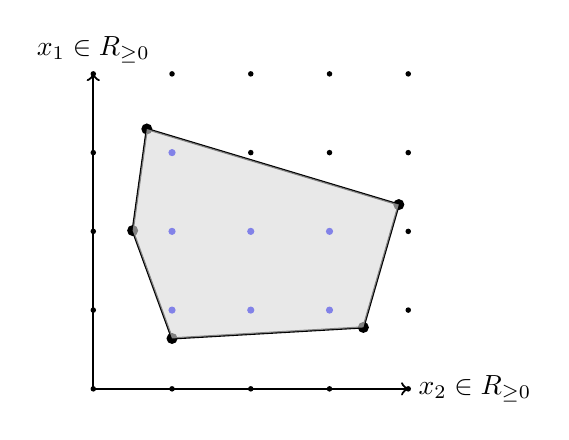
\begin{tikzpicture}[scale=1.0]
					% Grid
					\draw[->,thick] (0,0)--(4,0) node[right]{$x_2 \in \mathbb{R}_{\geq 0}$};
					\draw[->,thick] (0,0)--(0,4) node[above]{$x_1 \in \mathbb{R}_{\geq 0}$};
					
					% Beschriftung der Nebenbedingungen
					\draw[thick] (1,0.64)--(3.43,0.78);
					\draw[thick] (3.43,0.78)--(3.88,2.34);
					\draw[thick] (3.88,2.34)--(0.68,3.3);
					\draw[thick] (0.68,3.3)--(0.5,2.01);
					\draw[thick] (0.5,2.01)--(1,0.64);
					
					% Draw Points
					\fill (1,0.64) circle (2pt);
					\fill (3.43,0.78) circle (2pt);
					\fill (3.88,2.34) circle (2pt);
					\fill (0.68,3.3) circle (2pt);
					\fill (0.5,2.01) circle (2pt);
					
					\foreach \x in {0, 1, 2,3,4} {
						\foreach \y in {0, 1, 2,3,4} {
							\fill (\x, \y) circle (1pt);
						}
					}
					
					\fill[blue] (1,1) circle (1.3pt);
					\fill[blue] (2,1) circle (1.3pt);
					\fill[blue] (3,1) circle (1.3pt);
					\fill[blue] (1,2) circle (1.3pt);
					\fill[blue] (2,2) circle (1.3pt);
					\fill[blue] (3,2) circle (1.3pt);
					\fill[blue] (1,3) circle (1.3pt);
					
					% Zulässiger Bereich (grau hinterlegt)
					\fill[gray!30,opacity=0.6] 
					(1,0.64) 
					-- (3.43,0.78) 
					-- (3.88,2.34) 
					-- (0.68,3.3) 
					-- (0.5,2.01)
					-- cycle;
					
					% Drei rechtwinklige Striche am Ende
					%\foreach \i in {-0.2, 0, 0.2} {
						%	\draw[thick] 
						%	($ (3,0) + (\i,0) $) -- 
						%	($ (3,0) + (\i,0) + (45:0.2) $); % 45° ist senkrecht zur Linie (315° Linie)
						%}
				\end{tikzpicture}
			\end{minipage}%
			\begin{minipage}{0.45\textwidth}
				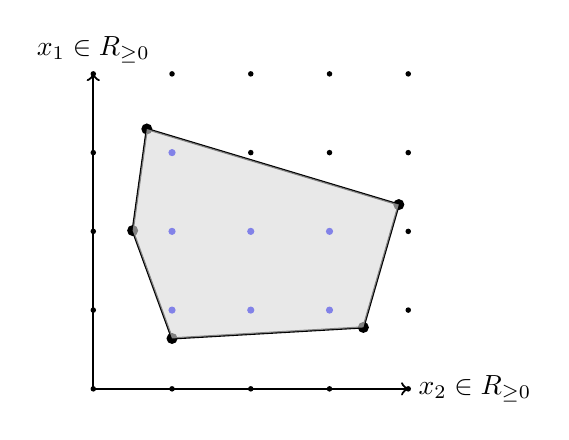
\begin{tikzpicture}[scale=1.0]
					% Grid
					\draw[->,thick] (0,0)--(4,0) node[right]{$x_2 \in \mathbb{R}_{\geq 0}$};
					\draw[->,thick] (0,0)--(0,4) node[above]{$x_1 \in \mathbb{R}_{\geq 0}$};
					
					% Beschriftung der Nebenbedingungen
					\draw[thick] (1,0.64)--(3.43,0.78);
					\draw[thick] (3.43,0.78)--(3.88,2.34);
					\draw[thick] (3.88,2.34)--(0.68,3.3);
					\draw[thick] (0.68,3.3)--(0.5,2.01);
					\draw[thick] (0.5,2.01)--(1,0.64);
					
					% Draw Points
					\fill (1,0.64) circle (2pt);
					\fill (3.43,0.78) circle (2pt);
					\fill (3.88,2.34) circle (2pt);
					\fill (0.68,3.3) circle (2pt);
					\fill (0.5,2.01) circle (2pt);
					
					\foreach \x in {0, 1, 2,3,4} {
						\foreach \y in {0, 1, 2,3,4} {
							\fill (\x, \y) circle (1pt);
						}
					}
					
					\fill[blue] (1,1) circle (1.3pt);
					\fill[blue] (2,1) circle (1.3pt);
					\fill[blue] (3,1) circle (1.3pt);
					\fill[blue] (1,2) circle (1.3pt);
					\fill[blue] (2,2) circle (1.3pt);
					\fill[blue] (3,2) circle (1.3pt);
					\fill[blue] (1,3) circle (1.3pt);
					
					% Zulässiger Bereich (grau hinterlegt)
					\fill[gray!30,opacity=0.6] 
					(1,0.64) 
					-- (3.43,0.78) 
					-- (3.88,2.34) 
					-- (0.68,3.3) 
					-- (0.5,2.01)
					-- cycle;
					
					% Drei rechtwinklige Striche am Ende
					%\foreach \i in {-0.2, 0, 0.2} {
						%	\draw[thick] 
						%	($ (3,0) + (\i,0) $) -- 
						%	($ (3,0) + (\i,0) + (45:0.2) $); % 45° ist senkrecht zur Linie (315° Linie)
						%}
				\end{tikzpicture}
			\end{minipage}
			\caption{Solution space of a linear program highlighted in gray. Point highlighted in blue represent the solution space of the corresponding integer linear program.}
			\label{fig:prelims:linear:solspace:unbounded}
		\end{figure}
		\todo{unbounded on right}
		
		Linear programming is widely used in various fields such as operations research, economics, engineering, and logistics, due to its efficiency in solving large-scale real-world optimization problems. Algorithms such as the Simplex Method and Interior Point Methods are commonly used to solve LP problems efficiently.
		The simplex algorithm in particular is widely used in practice because of its efficiency on most problems, even though its worst-case complexity is exponential-time on certain families of problems depending on the chosen pivot-rule. \todo{cite}
		However, on most problems the simplex algorithm only takes a polynomial number of steps to terminate.
		
		\subsection{Mixed-Integer Programs}
			%
			\begin{alignat*}{3}
				&z^*_{LP} \; &={}	\min	&\quad  c^T && \mathbf{x} \\
				&				  		& \text{s.t.} & \quad A && \mathbf{x} \geq b \\
				&						&					 &					&& \mathbf{x} \in \mathbb{Z}_{\geq 0}
			\end{alignat*}
			%
			
	
	\section{Dantzig-Wolfe Decomposition}
	% 3 Seiten
	
		\clearpage
		A\clearpage
		A\clearpage
	
	\section{Graph Theory}
	% 2 Seiten
	
		\clearpage
		A\clearpage
	
	\section{Partition Refinement}
	% 2 Seiten
		Partition refinement is a fundamental concept in computer science, particularly relevant in fields such as automata theory, graph theory and model checking.
		A \textit{partition} refers to a decomposition of a set $U$ into disjoint, non-empty subsets $\{ A_1, A_2, \ldots, A_k \}$, called \textit{cells} or \textit{blocks}, such that:
		\begin{equation*}
			\bigcup^k_{i=0} A_i = U \; \mathrm{and} \; \forall i \neq j: A_i \cap A_j = \emptyset
		\end{equation*}
		A partition $\pi = \{ A_1, A_2, \ldots, A_k \}$ of a set $U$ is called a refinement of a partition $\pi' = \{ B_1, B_2, \ldots, B_m \}$, iff
		\begin{equation*}
			\forall A_i \in \pi \;\; \exists B_j \in \pi' : A_i \subseteq B_j
		\end{equation*} 
		As a special case, a partition is a refinement of itself.
		More informally, partition $\pi'$ must reflect a \enquote{finer} classification of the elements than in $\pi$. 
		
		Partition refinement refers to an \textit{iterative} process that refines a given initial partition of a set over the course of multiple iterations.
		Given a splitter-function $f: U \mapsto Q$ which maps every element of $U$ to some element of an arbitrary target set $Q$, an initial partition $\pi_{\mathrm{init}}$ the goal is typically to find the coarsest partition $\pi_f = \{ A_1, A_2, \ldots, A_k \}$ of $U$ such that the following two properties hold:
		
		\begin{enumerate}
			\item The partition $\pi_f$ is a refinement of the initial partition $\pi_{\mathrm{init}}$
			\item $\forall A_i \in \pi_f \; \forall a, b \in P_i: f(a) = f(b)$, that is, the function $f$ can intuitively be thought of a function expressing a certain \enquote{property} for each element. Elements with different properties cannot be part of the same cell and must be separated from each other during the refinement process.
		\end{enumerate}
		
		Furthermore, the underlying problem structure to which partition refinement is applied, as well as the type of splitter function used, are not inherently restricted. In practice, however, many problems can be reformulated or encoded as graphs, where the function $f$ captures a vertex property.
		For instance, in deterministic finite automaton (DFA) minimization, partition refinement is used to iteratively distinguish states by observing the equivalence classes of their transitions (Hopcroft's algorithm): two states are grouped together only if, for every input symbol, their transitions lead into the same partition class; in graph isomorphism testing, it could encode vertex degrees or local neighborhood structures; and in Markov decision processes (MDPs), $f$ might reflect the expected reward or transition behavior.
		These encodings allow partition refinement to exploit structural symmetries and behavioral equivalences in a wide range of domains, especially if problems in that domain can be encoded as graphs.
		
		For the purposes of this work, $f$ will usually represent a function structurally similar to a \textit{connection function} as it used in many graph automorphism packages.
		Given a graph $G = (V, E)$, then we define two types of connection function as follows:
		\begin{align}
			f_{\mathrm{count}}(v, X_{\mathrm{ind}}) &= \left| \{ v' \in V \mid \forall (v, v') \in E, v' \in X_{\mathrm{ind}} \} \right| \label{eq:prelims:pref:count} \\
			f_{\mathrm{exists}}(v, X_{\mathrm{ind}}) &= \begin{cases}
				1 & \left| \{ v' \in V \mid \forall (v, v') \in E, v' \in X_{\mathrm{ind}}   \} \right| > 0 \label{eq:prelims:pref:exists} \\
				0 & \mathrm{else}
			\end{cases}
		\end{align}
		
		Functions \ref{eq:prelims:pref:count} and \ref{eq:prelims:pref:exists}
		
		\begin{algorithm}[ht!]
			\centering
			\begin{algorithmic}
				\While{Test}
				\EndWhile
			\end{algorithmic}
			\caption{Partition refinement algorithm}
			\label{algo:prelims:refinement}
		\end{algorithm}
	
		Furthermore, if the underlying graph is bipartite and the splitter-function is expressing a vertex-property, i.e., 
	
		\clearpage
	
	\section{Surprise and Entropy}
	
		\begin{figure}[ht!]
			\centering
			\includesvg[scale=0.82]{Bilder/DrawIO/entropy}
			\caption{Entropy is measure of \enquote{surprise} and it increases with decreasing probability. On the left side, both colors are evenly distributed, so drawing either one is equally surprising. On the right side, drawing a red ball from the set of elements would be very surprising, because the probability is only $\frac{1}{12}$. But because this event is so unlikely, one does \textit{not expect} to be surprised. As a result, the expected surprise - that is, the entropy - is low.}
			\label{figure:prelim:entropy}
		\end{figure}
	
		The \textit{information value} or \textit{surprisal} of an event $E$ is defined as
		\begin{equation}
			I(E) = \log_b \left( \frac{1}{p(E)} \right) = - \log_b \left( p(E) \right)
		\end{equation}
		It increases as the probability of the event $p(E)$ decreases.
		Intuitively, if the probability is close to $1$, then one wouldn't be surprised if this event actually occurred, so the surprisal is close to $0$.
		
		The \textit{entropy}, or \textit{expected surprise}, $H(X)$ of a discrete random variable $X$ which takes values in the set $\mathcal{X}$ is defined by equation \ref{eq:prelims:entropy} \cite{coverElementsInformationTheory2006}.
		\begin{equation}
		\label{eq:prelims:entropy}
			H(X) =  \sum_{x \in \mathcal{X}} p(x) I(X) = - \sum_{x \in \mathcal{X}} p(x) \log_b p(x)
		\end{equation}
		where $p(x) \coloneq \mathbb{P}[X = x]$.
		
		If not specified any further, the base $b$ of the logarithm is assumed to be $2$.
		In chapter \todo{ref} these concepts will be used to define a heuristic scoring system based on constraint names.
